\chapter{Gaussian Processes}\label{sec:gp}
A vast number of regression methods has been proposed in the machine learning 
literature. In this work I use Gaussian Processes as these have been 
successfully used in a number of studies related to spatial and environmental 
monitoring including the modeling of gas distributions 
\parencite[e.\,g.][]{Stranders:2008wl, Marchant:2012wb, Stachniss:2008vz}.  
Gaussian Processes exhibit a number of desirable features. They are 
non-parametric and non-linear. Therefore, they do not require any assumptions 
about the class of underlying functions or limitations of the search space.  
Also, they provide an estimate of the predictive uncertainties which can be used 
for a natural exploration-exploitation trade-off.

In the remainder of this chapter the essentials of Gaussian Process regression 
will be discussed.  A more thorough introduction can be found in 
\textcite{Rasmussen:2006vz}.

Let $X = \{\vc x_i | i = 1, \dots, n\}$ be a set of training inputs and $\vc 
y = (y_1, \dots, y_n)\Tr$ a vector of targets. The individual targets are 
assumed to follow $y_i = f(\vc x_i) + \eta$ with additive noise $\eta \sim 
\mathcal{N}(0, \sigma\ped{n}^2)$. The complete set of training data will be 
denoted with $\mathcal{D} = \{(\vc x_i, y_i) | i = 1, \dots, n\}$. We want to 
learn the function $f(\vc x)$ from this training data.

A \newterm{Gaussian Process}
\begin{equation}
    f(\vc x) \sim \mathcal{GP}(m(\vc x), k(\vc x, \vc x'))
\end{equation}
imposes a multivariate Gaussian distribution on the space of functions $f(\vc 
x)$. It is completely specified by the mean function $m(\vc x)$ and covariance 
function $k(\vc x, \vc x')$. Usually, though not necessarily, the mean function 
is taken to be zero. In most scenarios the choice of the covariance function is 
much more interesting as it controls features like the smoothness of the 
predicted underlying function. I will discuss this topic regarding the modeling 
problem on hand in Section~\ref{sec:covfn}.

We can now formulate the joint Gaussian prior distribution of the observed 
training targets and the predicted values $\vc f_*$ at unseen locations $X_*$ 
(assuming $m(\vc x) = 0$):
\begin{equation}
    \left[ \begin{array}{c}\vc y \\ \vc f_* \end{array} \right]
    \sim\mathcal{N}\!\del{\vc{0}, \sbr{\begin{array}{cc} K(X, X) 
                + \sigma\ped{n}^2 \mat I & K(X, X_*) \\ K(X_*, X) & K(X_*, X_*) 
            \end{array}}}
\end{equation}
Here $K(X, X')$ are matrices with the elements $(i, j)$ being the covariances 
$k(\vc x_i, \vc x'_j)$ evaluated for all pairs $\vc x_i \in X$ and $\vc x'_j \in 
X'$. In the following $\tilde{\mat K} = K(X, X) + \sigma\ped{n}^2 \mat I$ will 
be used as a shorter notation. By conditioning on the observations the 
predictive distribution for $\vc f_*$ is obtained as
\begin{align}
    \vc f_* | X, \vc y, X_* &\sim \mathcal{N}(\bar{\vc f_*}, \cov(\vc 
    f_*))\text{, with}\\
    \bar{\vc f_*} &= \mu(X_*) = K(X_*, X)\tilde{\mat K}^{-1} \vc y\text{,} 
    \label{eqn:meanpred} \\
    \cov(\vc f_*) &= K(X_*, X_*) - K(X_*, X)\tilde{\mat K}^{-1}K(X, X_*) 
    \label{eqn:covpred} \\
    \sigma^2(X_*) &= \diag(\cov(\vc f_*)) \text{.}
\end{align}
See Figure~\ref{fig:ex-gp-main} for a visualization of an example Gaussian 
process.

\begin{figure}
    \centering
    \subfigure[]{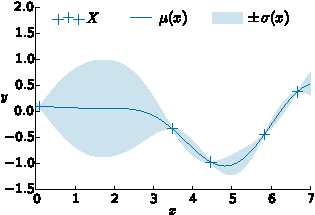
\includegraphics{plots/gp}\label{fig:ex-gp}}\hspace{0.5cm}%
    \subfigure[]{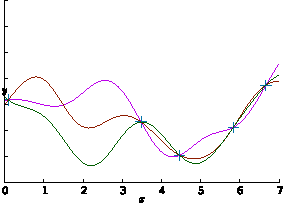
\includegraphics{plots/gp_sample}\label{fig:ex-gp-sample}}
    \caption[Gaussian process example]{Example of a one-dimensional Gaussian 
        process (using the squared exponential covariance function with 
        a length scale of 1, $\sigma\ped{n}^2 = 0$) conditioned on five training 
        points $X$: \subref{fig:ex-gp} shows the mean $\mu(x)$ and predictive 
        standard deviation $\sigma(X_*)$; \subref{fig:ex-gp-sample} shows three 
        functions sampled from the process.}\label{fig:ex-gp-main}
\end{figure}

Even though $\tilde{\mat K}$ is a symmetric, positive-definite matrix it can be 
ill-conditioned\footnote{The condition $\kappa(\mat A)$ of a matrix $\mat A$ is 
    defined as $\kappa(\mat A) = \|\mat A\| \|\mat A^{-1}\|$. Using the 
    $L^2$-norm this corresponds to $\kappa(\mat A) = \lambda_1/\lambda_n$,
    the ratio of the largest eigenvalue $\lambda_1$ and the smallest one
    $\lambda_n$. If the condition number $\kappa(\mat A)$ is too large, the 
    matrix is near-singular and ill-conditioned.} and lead to numerical 
instabilities. This happens especially for close-by input data points as they 
occur in a sequential scenario like the plume modeling here.

There are two commonly implemented approaches to counteract the problem of 
ill-conditioning \parencite[cp.][]{Sacks:1989cv, Neal:1997tj, Booker:1999wz, 
    Gramacy:2008es}. Firstly, instead of using a general matrix inversion 
algorithm one can utilize the symmetry and positive-definiteness of 
$\tilde{\mat{K}}$ by doing a Cholesky decomposition. This yields a lower, 
triangular matrix $\mat L$ satisfying $\tilde{\mat K} = \mat L\mat L\Tr$. The 
inverse can then be calculated as $\tilde{\mat K}^{-1} = (\mat L^{-1})\Tr \mat 
L^{-1}$.  Secondly, a well conditioned $\tilde{\mat K}$ can be ensured by adding 
a nugget $g > 0$ (also known as jitter) to the diagonal of the covariance 
matrix. This will increase all eigenvalues by the same value and thus improve 
the condition.  The addition of a nugget can also be seen as increasing the 
noise variance $\sigma\ped{n}^2$ and thus allowing the Gaussian Process to match 
the target less precisely and to become smoother.

\section{Online Updates}\label{sec:onlineup}
A naive implementation requires a $O\!\del[1]{\del[0]{n + N}^3}$ matrix 
inversion whenever new data points are added to the Gaussian Process with $N$ 
being the total number of data points collected so far and $n$ being the number 
of new data points.  However, it is possible to do online updates where only an 
$n \times n$ matrix has to be inverted.  This reduces the complexity of the 
matrix inversion to $O(n^3)$ and the overall complexity including the necessary 
matrix multiplications to $O(n \max\{n^2, N^2\})$.

Let us denote the set of inputs already trained on with $X$ and the set of 
inputs to add as $X'$. The block covariance matrix after adding these new inputs 
will be
\begin{equation} \label{eqn:tilde_K_prime}
    \tilde{\mat K}' = \left[ \begin{array}{cc}
            \tilde{\mat K} & K(X, X') \\ K(X', X) & K(X', X') 
            + \sigma\ped{n}^2\mat I
        \end{array}
    \right]\text{.}
\end{equation}
The Cholesky factorization can also be written with block matrices
\begin{equation}
    \tilde{\mat K}' = \mat L' {\mat L'}\Tr = \left[
        \begin{array}{cc}
            \mat L & \mat 0 \\ \mat A & \mat B
        \end{array}
    \right] \left[
        \begin{array}{cc}
            \mat L\Tr & \mat A\Tr \\ \mat 0 & \mat B\Tr
        \end{array}
    \right] = \left[
        \begin{array}{cc}
            \mat L \mat L\Tr & \mat L \mat A\Tr \\ \mat A \mat L\Tr & \mat A \mat 
            A\Tr + \mat B \mat B\Tr
        \end{array}
    \right]
\end{equation}
and comparison with equation~(\ref{eqn:tilde_K_prime}) gives the following 
relations:
\begin{align}
    \mat A &= K(X', X) \del[1]{\mat L\Tr}^{-1} \\
    \mat B \mat B\Tr &= K(X', X') + \sigma\ped{n}^2\mat{\mathrm{I}} - K(X', 
    X)\tilde{\mat{K}}^{-1}K(X, X')
\end{align}
As $\mat B \mat B\Tr$ is symmetric, positive-definite it is possible to obtain 
$\mat B$ also by a Cholesky decomposition.
With the inverse of a block matrix \parencite[45]{Petersen:2008wc} we obtain the 
following relation for the inverse of the updated Cholesky factor:
\begin{equation}
    \mat L'^{-1} = \left[
        \begin{array}{cc}
            \mat L^{-1} & \mat 0 \\ -\mat B^{-1} K(X', X)\tilde{\mat K}^{-1} 
            & \mat B^{-1}
        \end{array}
    \right]\label{eqn:invChol}
\end{equation}

\section{Sparse Approximations}
Despite online updates there is a quadratic increase in the complexity with 
adding more training data points to a Gaussian process. This efficiency problem 
can be alleviated by using a sparse approximation. A number of different methods 
has been proposed \parencites[chapter~8 
in][]{Rasmussen:2006vz}{QuinoneroCandela:2005wp}. Unfortunately, these methods 
usually assume that all training data is already accessible which is not the 
case in an online scenario. An exception to this is the online approximation by 
\textcite{Csato:2002fp}.

They replace the inverse covariance matrix $\tilde{\mat K}_t^{-1}$ in 
Equation~\ref{eqn:covpred} after $t$ updates with $-\mat C_t$. Normal (full) 
online updates are performed as discussed in the previous section by updating 
$-\mat C_t$ respectively the Cholesky factor $\mat L_t^{-1}$.\footnote{The 
    original paper formulates the update a bit different. The equivalence for 
    full updates is shown in Appendix~\ref{sec:sparse-gp-apdx}.} If, however, 
the ``novelty''
\begin{equation}
    \tilde{\sigma}^2_{t+1} = k(\vc x_*, \vc x_*) + \sigma\ped{n}^2 
    - K\!\del{\{\vc x_*\}, X_t} \tilde{\mat K}_t^{-1} K\!\del{X_t, \{\vc x_*\}}
\end{equation}
of a new input $\vc x_*$ is below a threshold $\epsilon\ped{tol}$, a reduced 
update will be performed. The reduced update leaves the size of $\mat C_t$ 
unchanged.

All inputs used for a full update are called basis vectors and constitute the 
set~$\mathcal{BV}$. The size of this set can be limited by deleting the basis 
vector with the smallest error whenever the limit is exceeded. The error 
associated with the $i$-th basis vector is given by
\begin{equation}
    e_i = \frac{\abs[1]{\del[1]{\tilde{\mat K}_{t+1}^{-1} 
                \vc{y}}_i}}{\del[1]{\tilde{\mat{K}}_{t+1}^{-1}}_{ii}} \text{.}
\end{equation}

The basis vector deletion requires downdating the approximate covariance matrix 
$-\mat C_{t+1}$ and performing a reduced updated with the deleted basis vector.  
Unfortunately, as shown in Appendix~\ref{sec:sparse-gp-apdx} the calculation of 
$-\mat C_t$ is based on the Cholesky factors and downdating based on Cholesky 
factorization or a matrix obtained from the factorization is known to be 
numerical unstable \parencite{Bjorck:1994dz}, especially when the correlation of 
the training inputs is high. Using other factorizations like the QR 
factorization a more stable downdating algorithm can be obtained.  However, this 
comes at the cost of the initial factorization being numerical more unstable.  
Also, it would be possible to directly downdate $\tilde{\mat{K}}_{t+1}$ and 
recalculate the Cholesky factorization. Yet, this leads to cubic instead of 
quadratic complexity for downdating.

It turned out that these issues with numerical stability do not make this sparse 
online approximation a viable option for plume distribution estimation. The 
collected samples are highly correlated and make downdating the Cholesky factor 
too unstable, while using a more stable method impairs efficiency below the 
non-sparse Gaussian process level. By resigning from deleting basis vector and 
only using reduced updates based on the novelty $\tilde{\sigma}^2_{t+1}$ not 
much is gained. The novelty only considers the spatial relation of inputs, but 
not the actual error in prediction at those locations. Hence, one would either 
still use almost all data for full updates or use not enough full updates in 
areas of high concentration where a close sampling is necessary. Luckily, the 
performance of the non-sparse Gaussian processes was sufficient as at most only 
a few thousand training inputs were used.

\section{Covariance Functions}\label{sec:covfn}
The choice of the covariance function determines the assumptions about the most 
probable functions learned with a Gaussian process. Hence, it is important for 
reaching the best performance.  In this chapter, I will discuss some widely used 
covariance functions and considerations to take into account. A more thorough 
discussion including further covariance functions is to be found in 
\textcite[Chapter 
4]{Rasmussen:2006vz} on which this section is based.

A valid covariance function $k(\vc x, \vc x')$ is a kernel satisfying 
positive-definiteness
\begin{equation}
    \int f(\vc x) k(\vc x, \vc x') f(\vc x') \dif \vc x \dif \vc x' \geq 
    0 \text{.}
\end{equation}
This ensures that the kernel's Gram matrix for a set of inputs $\cbr{x_i 
    | i = 1, \dots, n}$ with entries $\mat K_{ij} = k(\vc x_i, \vc x_j)$ is also 
positive-definite and therefore a valid, invertible covariance matrix.

The \newterm{smoothness} of the Gaussian process is determined by the covariance 
function.  This is formalized in the notion of how many times the process $f(\vc 
x)$ is \newtermAbbrev{mean square}{MS}\newterm{ differentiable}.  It is 
differentiable if the mean square limit denoted by $\mslim$ in the mean square 
derivative exists. The MS derivative is given by
\begin{equation}
    \dpd{f(\vc x)}{x_i} = \mslim_{h \rightarrow 0} \frac{f(\vc x + h\vcc e_i) 
    - f(\vc x)}{h}
\end{equation}
for the $i$-th direction with the unit vector $\vcc e_i$.

%defined in \textcite[81]{Rasmussen:2006vz} in the following way: ``Let $x_1, 
%x_2, \dots$ be a sequence of points and $x_*$ be a fixed point in $\mathbb{R}^D$ 
%such that $\abs{x_k - x_*} \rightarrow 0$ as $k \rightarrow \infty$. Then 
%a process $f(x)$ is continuous in mean square at $x_*$ if 
%$\mathbb{E}[\abs[0]{f(x_k) - f(x_*)}^2] \rightarrow 0$ as $k \rightarrow 
%\infty$. If this holds for all $x_* \in A$ where $A$ is a subset of 
%$\mathbb{R}^D$ then $f(x)$ is said to be continuous in mean square (MS) over 
%$A$.''

\subsection{Stationary Covariance Functions}
A kernel which is only a function of $\vc x - \vc x'$ is called 
\newterm{stationary} and is invariant to translations. Furthermore, it is 
\newterm{isotropic} if it is a \abbrev{radial basis function}{RBF} $k(r)$ with 
    $r = \abs{\vc x - \vc x'}$.  An isotropic kernel is invariant to all rigid 
    motions.

For stationary kernels the smoothness properties of the resulting Gaussian 
process can be easily obtained: It is $k$-times MS differentiable if at $\vc 
x = \vc 0$ the $2k$-th order partial derivatives $\partial^{2k} k(\vc x) 
/ \partial x_{i_1}^2 \dots \partial x_{i_k}^2$ exist and are finite. Thus, the 
process smoothness is essentially determined by the kernel properties around 
$\vc 0$.

A common default choice is the \newtermAbbrev{squared exponential}{SE} kernel 
    defined as
\begin{equation}
    k\ped{SE}(r) = \sigma\ped{k}^2 \exp\!\del{-\frac{r^2}{-2\ell^2}}
\end{equation}
with the desired process variance $\sigma\ped{k}^2$ and length scale $\ell$. It 
produces infinitely MS differentiable Gaussian processes. This can, actually, be 
too smooth in many applications.

The \newterm{Mat\'ern class} of covariance functions allows to control the 
smoothness with a parameter $\nu$. Using the modified Bessel function $K_{\nu}$ 
it is given by
\begin{equation}
    k_{\nu}(r) = \sigma\ped{k}^2 \frac{2^{1-\nu}}{\Gamma(\nu)} 
    \del{\frac{r\sqrt{2\nu}}{\ell}}^{\nu} 
    K_{\nu}\!\del{\frac{r\sqrt{2\nu}}{\ell}} \text{.}
\end{equation}
The resulting Gaussian process will be $k$ times MS differentiable for $k 
< \nu$. The parameter $\ell$ denotes again the characteristic length scale.

Typically, only the kernels with $2\nu \in \cbr{1, 2, 3}$ are used.  Usually it 
is not possible to tell which kernel leads to a better fit for larger $\nu$ from 
the noisy data.  To simplify the function half-integer values are used as the 
kernel functions will become:
\begin{align}
    k_{5/2}(r) &= \sigma\ped{k}^2 \del{1 + \frac{r\sqrt{5}}{\ell} 
        + \frac{5r^2}{3\ell^2}} \exp\!\del{-\frac{r\sqrt{5}}{\ell}} \\
    k_{3/2}(r) &= \sigma\ped{k}^2 \del{1 + \frac{r\sqrt{3}}{\ell}} 
    \exp\!\del{-\frac{r\sqrt{3}}{\ell}} \\
    k_{1/2}(r) &= k_{\exp}(r) = \sigma\ped{k}^2 \exp\!\del{-\frac{r}{\ell}}
\end{align}
From these kernel functions $k_{\nu=1/2}(r)$ is also known as the 
\newterm{exponential kernel}. Furthermore, note that for $\nu \rightarrow 
\infty$ the squared exponential kernel is recovered. A plot comparing the 
different covariance functions can be found in Figure~\ref{fig:kernels}.

\begin{figure}
    \centering
    \subfigure[]{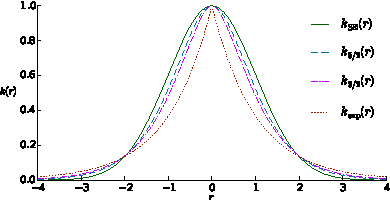
\includegraphics{plots/kernels}\label{fig:kernels-kern}}
    \subfigure[]{\includegraphics{plots/kernsamples}\label{fig:kernels-kernsamples}}
    \caption[Covariance functions]{Comparison of covariance functions.  
        \subref{fig:kernels-kern} Plot of stationary covariance functions with 
        $\sigma_k^2 = 1, \ell = 1$. \subref{fig:kernels-kernsamples} One 
        function sampled for each of the covariance functions from a Gaussian 
        Process prior with $m(\vc x) = 0$.}\label{fig:kernels}
\end{figure}

\subsection{Non-stationary Covariance Functions}
Many phenomena, including the concentrations of gas plumes, are not stationary.  
Already a Gaussian density function exhibits different optimal length scales.  
With a long length scale the predicted mean can considerably deviate from the 
target function as shown for positive $x$ in Figure~\ref{fig:gp-length-scale}.  
With a short length scale a good fit is obtained.  However, the predictive 
variance along the tail towards negative $x$ is overestimated as the actual rate 
of change in this area is low.

\begin{figure}
    \centering
    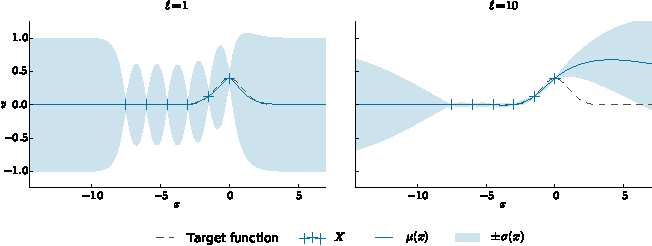
\includegraphics{plots/gp-lengthscale}
    \caption[Length scale influence]{Influence of the kernel length scale on the 
        Gaussian process. In both plots the Mat\'ern kernel with $\nu = 3/2$ was 
        used. On the left a short length scale of $\ell = 1$ was used, whereas 
        a longer length scale of $\ell = 10$ was used on the right.
    }\label{fig:gp-length-scale}
\end{figure}

Non-stationary covariance functions can lessen this problem. Moreover, they 
allow to model discontinuities at specific places. However, the usage of 
non-stationary covariance functions for the given plume modeling problem is far 
from straightforward and might need more prior knowledge than one is willing to 
assume (in simulations) or effectively has.  One would probably have to use 
different kernels depending on the scenario (wind/no wind, number of sources) 
and these would have to be parameterized with the source locations. Otherwise 
the non-stationarity of the kernel could not relate to the actual 
non-stationarity of the plume.

Methods for selecting such parameters will be discussed in the next section.  
Unfortunately, the cost of these methods grows with the number of parameters, 
which for non-stationary kernels will be larger than for stationary kernels.  
Matters are complicated even more as it is usually desirable to have 
a differentiable kernel to be able to use gradient-based optimizers. Moreover, 
in an active learning scenario there is a limited amount of data in the 
beginning making the correct estimation of parameters like the source position 
virtually impossible.

It also has to be taken into account that non-stationary kernels might not be 
agnostic to the structure of the modeled function. Such a covariance function 
will lead to better results if the function matches the structural assumptions 
of the kernel. However, if that is not the case, the results will probably be 
worse than with stationary kernels agnostic to the structure. Especially when 
modeling a plume distribution in a real world scenario one would have to 
consider a multitude of effects like obstacles and local changes in wind.  That 
might make it impossible to derive valid structural assumptions for using 
a non-stationary kernel.

\section{Hyper-parameter Selection}
Though Gaussian processes are non-parametric, the choice of the covariance 
function will introduce hyper-parameters $\vc \theta$ (i.\,e.~the length scale) 
which have to be set.  In the following I will discuss three methods for doing 
so.

With the \newterm{test set method} all data available $\mathcal{D}$ will be 
split into two sets $\mathcal{D}_0$ and $\mathcal{D}_*$. The set $\mathcal{D}_0$ 
is used to train Gaussian processes with different covariance functions and 
hyper-parameters. For each model the generalization error $E\ped{G}$ over the 
test set $\mathcal{D}_*$ will be evaluated and the parameters with the minimal 
generalization error will be chosen. The error measure can be chosen freely with 
respect to what should be considered a good model. The root mean square error is 
a typical choice (see also Chapter~\ref{sec:error}).

If the amount of available data is limited, it is common to use 
\newterm{$k$-fold cross validation} where $\mathcal{D}$ is split into $k$ 
disjoint subsets $\mathcal{D}_i$ of equal size and the generalization error will 
be calculated from $k$ different models using the respective $\mathcal{D}_i$ as 
test set and the other sets as training data.

The third possibility is to find $\argmax_{\vc \theta} p(\vc\theta | \vc y, X, 
\mathcal{H}_i)$, wherein
\begin{equation}
    p(\vc\theta | \vc y, X, \mathcal{H}_i) = \frac{p(\vc y | X, \vc\theta, 
        \mathcal{H}_i) p(\vc\theta | \mathcal{H}_i)}{p(\vc y | X, 
        \mathcal{H}_i)}
\end{equation}
consisting of the marginal likelihood $p(\vc y | X, \vc\theta, \mathcal{H}_i)$, 
a prior $p(\vc\theta | \mathcal{H}_i)$, a normalization factor $p(\vc y | X, 
\mathcal{H}_i)$, and a set of possible model structures $\mathcal{H}_i$. The 
normalization factor can be difficult to estimate 
\parencite[109]{Rasmussen:2006vz}. For that reason, even though it can more 
easily lead to overfitting, often only the marginal likelihood is optimized 
which is known as \newterm{type~\RN{2} maximum likelihood}. For a Gaussian 
process with $n$ training samples it is given by
\begin{equation}
    \ln p(\vc y | X, \vc\theta) = -\frac{1}{2}\del{\vc y\Tr \tilde{\mat{K}}^{-1} 
        \vc y + \ln \det \tilde{\mat K} + n \ln 2\uppi} \text{.}
\end{equation}
The three summands can be interpreted as the quality of the data fit $\vc y\Tr 
\tilde{\mat K}^{-1} \vc y$, model complexity $\ln \det \tilde{\mat K}$, and 
a normalization term $n \ln 2\uppi$. Hence, the optimization of the marginal 
likelihood includes an automatic trade-off of model complexity and data fit.

Optimizing the marginal likelihood has the advantage (in comparison to the test 
set method) that a gradient based optimizer can be used. The partial derivatives 
of the likelihood are given by
\begin{equation}
    \dpd{}{\theta_j} \ln p(\vc y | X, \vc\theta) = \frac{1}{2} 
    \del{\del{\tilde{\mat K}^{-1}\vc y \vc y\Tr \tilde{\mat K}^{-1} 
            - \tilde{\mat{K}}^{-1}} \dpd{\tilde{\mat K}}{\theta_j}} \text{.}
\end{equation}
Nevertheless, all methods require a complete retraining of the Gaussian process 
as for each update of the hyper-parameters $\tilde{\mat K}^{-1}$ has to be newly 
calculated.  Thus, in an online setting it is far more efficient to keep the 
hyper-parameters fixed or only update them occasionally.

\section{Active Learning and Bayesian Optimization}
A setting in which a learning algorithm can freely choose the next training 
input is called \newterm{active learning}. A general introduction to the topic 
is provided by \textcite{Settles:2009vo}. The \newtermAbbrev{Bayesian 
    optimization}{BO} framework provides a method well suited for active 
learning with Gaussian process. An extensive introduction to Bayesian 
optimization is given by \textcite{Brochu:2010um}.

In short Bayesian optimization is a method for finding the maximum of an 
objective function $f(\vc x)$. The only condition on $f(\vc x)$ is that it is 
Lipschitz continuous, meaning that a constant $C$ exists, such that
\begin{equation}
    \abs{f(\vc x) - f(\vc x')} \leq C \abs{\vc x - \vc x'} \text{.}
\end{equation}
A closed form expression of $f(\vc x)$ may be unknown and it might be costly to 
evaluate. Because of the latter, Bayesian optimization tries to keep the number 
of function evaluations small.

The general BO algorithm can be described as follows: Given the prior beliefs 
about the objective function $p(f)$ a sampling location $\vc x_t$ is chosen. The 
sample acquired at $\vc x_t$ is used to obtain a posterior according to Bayes' 
Theorem
\begin{equation}
    p(f|\mathcal{D}_{1:t}) \propto p(\mathcal{D}_{1:t} | f) p(f) \text{.}
\end{equation}
This posterior represents the updated beliefs about the objective function.

The beliefs about the objective function can be expressed using Gaussian 
processes. Adding further data points corresponds to obtaining an updated 
posterior. The complete BO algorithm with Gaussian processes is stated in 
Algorithm~\ref{algo:bo}.

\begin{algorithm}[t]
    \For{$t = 1, 2, \dots$}{
        Find $\vc x_t$ by optimizing the acquisition function over the GP\@: 
        $\vc x_t = \argmax_{\vc x} u(\vc x|\mathcal{D}_{1:t-1})$\;
        Sample the objective function: $y_t = f(\vc x_t) + \varepsilon_t$\;
        Augment the data $\mathcal{D}_{1:t} = \{\mathcal{D}_{1:t-1}, (\vc x_t, 
        y_t)\}$ and update the GP\@.
    }
    \caption{Bayesian optimization algorithm using a Gaussian Process. Taken 
        from \textcite[6]{Brochu:2010um}}\label{algo:bo}
\end{algorithm}

So far it is still open how the sampling location $\vc x_t$ is selected. For 
that an \newterm{utility} or \newterm{acquisition}\footnote{The terms will be 
    used interchangeable in the following.} function $u(\vc x)$ indicating the 
expected benefit for choosing $\vc x$ as next training sample is used.  Hence, 
the optimal choice is $\argmax_{\vc x} u(\vc x)$.  Equivalently, it is possible 
to use the negative of a loss function $u(\vc x) = - \lambda(\vc x)$. In the 
next section different possible acquisition functions will be discussed in the 
context of plume distribution modeling.

\subsection{Acquisition Functions}\label{sec:utility}
The choice of the acquisition function $u(\vc x)$ influences the 
exploration-exploitation trade-off and on which areas of the input space the 
learning will be focussed.  In the estimation of a plume distribution samples 
should be acquired mostly at places with high concentrations, but once such an 
area is well estimated further exploration should follow to possibly find 
further sources.

\Textcite{Marchant:2012wb} proposed the \newtermAbbrev{distance-based upper 
    confidence bound}{DUCB} for a scenario of environmental monitoring where 
ozone concentrations over US territory were to be measured:
\begin{equation}
    u\ped{DUCB}(\vc x) = \mu(\vc x) + s\ped{DUCB}(\vc y) \sbr{\kappa \cdot 
        \sigma^2(\vc x) + \gamma \cdot d(\vc x, \vc x')}
\end{equation}
The mean prediction $\mu(\vc x)$ and the predictive variance $\sigma^2(\vc x)$ 
are obtained directly from the Gaussian process, $d(\vc x, \vc x')$ denotes the 
Euclidean distance of $\vc x$ to the last sample location $\vc x'$. For ease of 
notation these functions are assumed to be unitless. Precisely this means that 
$\mu(\vc x)$ is divided by \si{\gram\per\meter\cubed}, $\sigma^2(\vc x)$ by 
\si{{\gram\squared\per\meter\tothe{6}}}, and $d(\vc x, \vc x')$ by \si{\meter}.

The parameter $\kappa$ controls the exploration-exploitation balance.  Higher 
values give more importance to decreasing the predictive variance and lead to 
more exploration.  The parameter $\gamma \leq 0$ adjusts the distance penalty.  
Favoring locations near to the current UAV position might decrease the distance 
travelled and save energy as well as time.  The original DUCB formulation by 
\textcite{Marchant:2012wb} did not include the scaling factor $s(\vc y)$. To 
match that formulation it has to be set to $s\ped{DUCB}(\vc y) = 1$. Another 
possible choice will be discussed below.

Though, the ozone concentration scenario appears to be similar to the plume 
modeling problem at hand one should note a certain difference. The ozone 
concentration is a smooth distribution as \textcite{Marchant:2012wb} used the 
squared exponential covariance function to obtain reasonable results. In 
opposite to that, the spatial distribution of a gas plume is much more localized 
\parencite[this was also noted by][]{Stachniss:2008vz}. Thus, I propose the 
\newtermAbbrev{plume distance-based upper confidence bound}{PDUCB} acquisition 
function inspired by DUCB, but adjusted:
\begin{multline}
    u\ped{PDUCB}(\vc x) = \del{1 - a} \cdot \ln\del{\mu_+(\vc x) + \varepsilon} 
    + a \cdot \ln \varepsilon \\ + s\ped{PDUCB}(\vc y) \sbr{\kappa \cdot 
        \del[1]{\sigma^2(\vc x) -  \sigma\ped{n}^2} + \gamma \cdot d^2(\vc x, 
        \vc x')}
\end{multline}
with
\begin{align}
    a &= \e^{-\mu_+(\vc x) / \varepsilon} \\
    \mu_+(\vc x) &= \max\cbr{0, \mu(\vc x)}
\end{align}

Using the logarithm of the process mean makes this utility function sensitive 
for small concentration changes in areas of low concentration. These can hint 
towards areas with higher concentration.  Being sensitive to the same absolute 
change for high concentrations is not as important. As the concentration might 
be equal to zero strict positiveness has to be explicitly ensured by a small 
$\varepsilon > 0$.  Also, semi-positiveness of the predictive mean has to be 
ensured.

It is desirable to have differentiable acquisition functions to be able to use 
gradient based optimizers. However, due to the logarithm the function would not 
be differentiable for $\mu(\vc x) \rightarrow 0$. Thus, it is weighted with $(1 
- a)$ and faded out to $\ln \varepsilon$ to restore differentiability (proof in 
Appendix~\ref{sec:pducb-diff}).

The noise variance $\sigma\ped{n}^2$ is subtracted from the predictive variance 
as $\sigma^2(\vc x) \geq \sigma\ped{n}^2$ and this way $\kappa$ needs no 
adjustment if the noise variance changes.

A further change in PDUCB compared to DUCB is the squaring of the distance which 
will reduce the penalty around $\vc x'$ (while increasing it further away).  
This should be advantageous as the unsquared distance function tends to force 
$\vc x$ much closer to $\vc x'$. Though the next sample should be near to $\vc 
x'$, it should not be too close to $\vc x'$.  Otherwise, not much new 
information would be gained due to the spatial correlation.

Apart from some explicit values, \textcite{Marchant:2012wb} do not discuss how 
to choose the parameters $\kappa$ and $\gamma$. Nevertheless, some observations 
can be made for both DUCB and PDUCB\@. Firstly, one should choose $\kappa \cdot 
\max \sigma^2(\vc x) > \max \mu(\vc x)$. Otherwise, one can get stuck in a local 
maximum as the mean term might get larger than the predictive variance term 
anywhere in the input space. Even though it can be a good strategy to exploit 
maxima first, exploration should continue once the distribution around the 
maximum is accurately known. A too small $\kappa$ is also problematic as it 
prevents any exploitation. Secondly, $\abs{\gamma}$ should not be too large or 
the distance penalty would dominate and also lead to one getting stuck in one 
position $\vc x = \vc x'$. Thirdly, $\varepsilon$ influences the sensitivity for 
low concentrations and should therefore be small, but large enough to prevent 
numerical problems in the evaluation of the logarithm. A value of $\varepsilon 
= 10^{-30}$ seems to work well (see Chapter~\ref{sec:exp}).  Finally, it should 
be noted that PDUCB needs a different scaling $s\ped{PDUCB}(\vc y)$ because the 
logarithm of the mean prediction is used.  Assuming $\mu(\vc x)$ will be in the 
range \numrange{0}{1}, the range of the logarithmic mean prediction term will be 
$\ln(1) - \ln(\varepsilon) \approx 70$.  Thus, setting $s\ped{PDUCB}(\vc y) 
= 70$ will make the other parameters of DUCB and PDUCB roughly comparable.

Typically, one knows the spatial dimensions of the input space which allows to 
estimate a reasonable $\gamma$ in relation to $\kappa$ as the maximal predictive 
variance is given by $\sigma\ped{n} + \sigma\ped{k}$.  However, the maximal $\vc 
y$ determining $\max \mu(\vc x)$ which is important for the absolute values of 
$\gamma$ and $\kappa$ in relation to the prediction mean might not be known in 
advance.  Thus, it would be helpful to set these parameters automatically from 
$\vc y$, the data seen so far.  This can be done by setting the scaling factor 
$s(\vc y)$ defined for the respective acquisition functions as
\begin{align}
    s\ped{DUCB}(\vc y) &= \max \vc y \cdot \si{\meter\cubed\per\gram} 
    \label{eqn:scale-ducb}\\
    s\ped{PDUCB}(\vc y) &= \ln(\max \vc y \cdot \si{\meter\cubed\per\gram} 
    + \varepsilon) - \ln \varepsilon \text{.} \label{eqn:scale-pducb}
\end{align}
The parameters $\kappa$ and $\gamma$ can then be set independently of the actual 
values of $\vc y$.

A third potential acquisition function, also balancing exploration and 
exploitation, can be derived from the work by \textcite{Osborne:2009tn}. They 
introduce a Bayesian approach for global optimization. Adopting their approach 
for a one-step look-ahead one first defines a loss function equal to the 
negative maximum after making a new observation
\begin{equation}
    \lambda\ped{GO} (y_*) = \left\{ \begin{array}{ll}-y_* & y_* > \eta \\ -\eta 
            & y_* \leq \eta \end{array} \right.
\end{equation}
with $\eta = \max \vc y$. From this the expected loss can be determined as
\begin{equation}\begin{split}
    \varLambda\ped{GO}(\vc x) &= \int \lambda\ped{GO}(y_*) p(y_* | \vc x, X, \vc 
    y) \dif y_* \\
    &= -\eta - \del{\mu(\vc x) - \eta} \varPhi\!\del{\eta; \mu(\vc x), 
        \sigma^2(\vc x)} - \sigma^2(\vc x) N\!\del{\eta; \mu(\vc x), 
        \sigma^2(\vc x)}
    \text{.}
\end{split}\end{equation}
In this equation $N(x; \mu, \sigma^2)$ and $\varPhi(x; \mu, \sigma^2)$ are the 
Gaussian probability density and respectively the Gaussian cumulative 
distribution function with mean $\mu$ and variance $\sigma^2$. Adding a distance 
penalty term to the negative of $\varLambda\ped{GO}(\vc x)$ gives the final 
utility function
\begin{align}\begin{split}
    u\ped{GO}(\vc x) &= -\varLambda\ped{GO}(\vc x) + \gamma \cdot d^2(\vc x, \vc 
    x') \\
    &= \eta + \del{\mu(\vc x) - \eta} \varPhi\!\del{\eta; \mu(\vc x), 
        \sigma^2(\vc x)} + \sigma^2(\vc x) N\!\del{\eta; \mu(\vc x), 
        \sigma^2(\vc x)}\\ &\quad+ \gamma \cdot d^2(\vc x, \vc x') \text{.}
\end{split} \end{align}
This approach can be extended to perform a look-ahead of multiple steps.  
However, this was not done here.

In Figure~\ref{fig:acqfns} a graphical comparison of the proposed utility 
functions is given for a one-dimensional example. It can be seen that DUCB 
heavily focusses on the function maximum without much exploration in other 
areas. The GO acquisition function also acquires more samples around the 
maximum, but reduces the uncertainty more equally over the domain. In comparison 
to these two functions PDUCB seems to also focus around the maxima, but with 
a wider exploration around those. In Chapter~\ref{sec:cmputility} I will more 
closely look on how well these functions work to estimate a plume dispersion 
with different parameter choices.

\begin{figure}
    \centering
    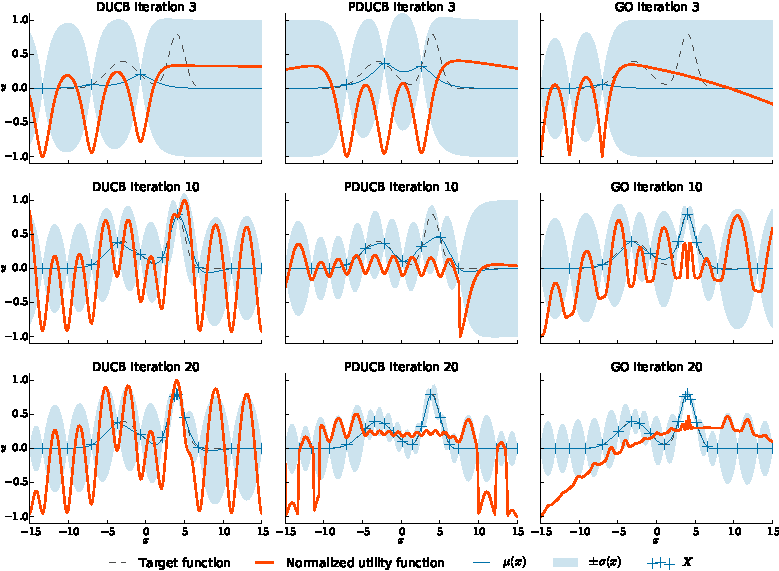
\includegraphics{plots/acqfns}
    \caption[Visualization of acquisition functions]{Visualization of 
    acquisition functions. The columns of the plot matrix correspond to the 
    three different acquisition functions (DUCB, PDUCB, GO) and the rows show 
    the state after 3, 10, and 
        20 iterations.  The utility functions were normalized by dividing by 
           $\max_{x \in \intcc{-15, 15}} \abs[0]{u(x)}$.
        The parameters used for these plots were $\kappa = 1.25$, $\gamma 
        = -0.0002$, $\varepsilon = 10^{-30}$, $s\ped{DUCB}(\vc y) = 1$, and 
        $s\ped{PDUCB}(\vc y) = 70$. The initial sample was always chosen at $x_0 
        = -7$.}\label{fig:acqfns}
\end{figure}

\subsection{Multiple UAVs}\label{sec:multiple-uavs}
Using more than one UAV might considerably speed up the estimation of a plume 
distribution. For that reason I propose a method to extend the target selection 
with an acquisition function $u(\vc x)$ to multiple UAVs. To not impair the 
performance of the original utility function one mobile robot will be selected 
as a \newterm{master UAV} and uses exactly $u(\vc x)$. Without loss of 
generality we can assign the index $i = 1$ to that UAV\@. For all other vehicles 
with $i > 1$ the following modified acquisition function
\begin{equation}
    u_i(\vc x) = u(\vc x) + \rho \sum_{j = 1,\ i \neq j}^n d^2(\vc x, \vc x_j)
\end{equation}
will be used where $\vc x_j$ is the position of the $j$-th UAV\@. This modified 
acquisition function basically introduces a penalty for locations close to other 
UAVs to spread them out.

\subsection{Initial Search Strategies}\label{sec:bootstrapping}
As long as no minimal concentration has been measured all of the proposed 
acquisition functions do not have a unique maximum. Though one could choose 
sampling locations randomly, this might take a long time until the plume gets 
discovered.  Hence, it is best to employ a more systematic search strategy in 
the beginning.

Here, three variations will be used. First, surrounding the area at a medium 
height.  Without noise this is sufficient to obtain enough information for 
a successful usage of the discussed acquisition functions.

Considering noise a second strategy is needed as measurements of low 
concentrations are not reliably anymore. This strategy, in the following called 
\newterm{complete search}, consists of surrounding the area at different heights 
until a criterion that a plume as been found is fulfilled. The criterion 
employed here is that the maximum of all concentration measurements $\max_i y_i$ 
for one surrounding has to be larger than $5\sigma(y_i)$ with $\sigma(y_i)$ 
being the standard deviation of the $y_i$.

This complete search may also take a long time before a plume has been found, 
but should be faster than random exploration. If the wind direction is known 
(which is not the case in the standard QRSim scenarios), a third strategy called 
\newterm{wind based search} can be used.  It improves the second strategy by not 
doing complete surrounds of the area, but only along the two area edges which 
are ``hit'' by the wind.  Those are the only two were the plume might be 
detected.

These bootstrapping strategies can be easily extended to multiple UAVs by 
assigning different heights to each one.

Most of the samples acquired during this bootstrapping process do not improve 
the estimation of the plume distribution. Thus, most of them were discarded to 
improve efficiency.  Only the measurements from surrounding the area for the 
last time before the plume was identified were used for the training of the 
Gaussian process.

